
\documentclass[12pt]{article}
% \documentclass{report}
% \documentclass[journal]{IEEEtran}

\usepackage{cite}
\usepackage{amsmath,amssymb,amsfonts}
\usepackage{algorithmic}
\usepackage{graphicx}
\usepackage{textcomp}
\usepackage{bm}

\usepackage[retainorgcmds]{IEEEtrantools}


\title{Bayesian Learning using a Non-Informative Prior over Finite-Dimensional Spaces}
\author{Paul Rademacher}
\date{October 20, 2017}


%\graphicspath{ {C:/Users/Paul/Documents/PhD/Dissertation/Documentation/Figures/} }
\graphicspath{ {Figures/} }

\DeclareMathOperator*{\argmin}{arg\,min}
\DeclareMathOperator*{\argmax}{arg\,max}


\begin{document}

\maketitle




\section{Introduction}

This report details a Bayesian perspective on stastical learning theory when both the input and outputs exist in finite dimensional spaces and a uniform prior distribution is used. To simplify the presentation, the first sections will assume that the predictions are not driven by any observable variable; subsequently, the results will be extended to the more practical case where we want to generate an estimate given observed data.

While the validity of Bayesian methods for statistical signal processing and machine learning has long been contended, the author believes it to be a justified approach that does not necessarily imply that the generative model is `random'; rather, it simply reflects the desire of the user to formulate risk as a weighted sum of learner performance across the space of models. 

The uniform, or `non-informative', prior is of specific interest because it reflects the user's lack of confidence that his/her data was generated using any specific distribution. Integrating a learner's risk with such a prior provides a Bayesian analogy to the ``No Free Lunch'' theorem; however, it will be shown that for a general loss metric, all learning functions \emph{do not} provide the same performance.

After examining the joint and conditional probability mass functions for the unobserved outputs and the training data, the results will be applied to two of the most common loss functions in machine learning: the squared error loss function (common for regression), and the 0-1 loss function (common for classification). Optimal learners will be presented and the loss as a function of space dimensions and volume of training data will be provided. Additionally, asymptotic results for these values will be discussed to provide insight into how well these learners perform for infinite input-output spaces and as the number of training examples increases. 




\section{Basic model: scalar estimate, no observations, identical decison space}


\subsection{Model}

In this simplified treatment, we want to design a learner to provide an estimate of unobserved ``output'' variable $\mathrm{y} \in \mathcal{Y} = \{ y_1, \ldots, y_M \}$ using $N$ observed training examples $\mathrm{D} \in \mathcal{D} = \mathcal{Y}^N$. It is assumed that the output and training data are independently and identically distributed according to an unknown probability mass function (PMF), 

\begin{equation}
\bm{\theta} = \begin{bmatrix} \theta_1 \\ \vdots \\ \theta_M \end{bmatrix} \in \bm{\Theta} 
= \left\{ \bm{\theta} \in {\mathbb{R}^+}^M: \sum_{m=1}^M \theta_m = 1 \right\} \;,
\end{equation}

such that,

\begin{equation}
\text{P}(y,D | \bm{\theta}) = \text{P}(y | \bm{\theta}) \prod_{n=1}^N \text{P}(D(n) | \bm{\theta}) \;,
\end{equation}

\begin{equation}
\text{P}_{\mathrm{y}}(y_m|\bm{\theta}) = \text{P}(\mathrm{y} = y_m | \bm{\theta}) = \theta_m
\end{equation}

\begin{equation}
\text{P}_{\mathrm{D}(n)}(y_m|\bm{\theta}) = \text{P}(\mathrm{D}(n) = y_m | \bm{\theta}) = \theta_m
\end{equation}


Our objective is to create a learning function $f: \mathcal{Y}^N \mapsto \mathcal{H}$ that minimizes a chosen risk function $\mathcal{R}(f) \in \mathbb{R}^+$.  The algorithm designer makes two decisions regarding how risk is calculated. First, he/she chooses a loss function $\mathcal{L}: \mathcal{H} \times \mathcal{Y} \mapsto \mathbb{R}^+$ that assigns a penalty dependent on both the unobserved output and the estimated value. Using this function, we calculate the conditional risk for a given model $\bm{\theta}$,

\begin{equation}
\mathcal{R}_{\bm{\Theta}}(f,\bm{\theta}) = \text{E}_{\mathrm{D}|\bm{\theta}} \left[ \text{E}_{\mathrm{y}|\bm{\theta}} \left[ \mathcal{L}(f(\mathrm{D}),\mathrm{y}) \right] \right] \;.
\end{equation}

Note the conditional independence between $\mathrm{y}$ and $\mathrm{D}$. The second choice the designer has is how to formulate a scalar risk from the set of conditional risks $\mathcal{R}_{\bm{\Theta}}(f,\cdot) : \bm{\Theta} \mapsto \mathbb{R}^+$. An obvious choice is to integrate over $\bm{\Theta}$; if the designer has some prior knowledge, a weighting function $w(\bm{\theta}) \in \mathbb{R}^+$ can be used, such that the full risk function is,

\begin{equation}
\mathcal{R}(f) = \int_{\bm{\Theta}} w(\bm{\theta}) \mathcal{R}_{\bm{\Theta}}(f,\bm{\theta})\mathrm{d}\bm{\theta} \;.
\end{equation}

Since affine transformation of an objective function will not change its minimizer, we can freely scale the non-negative weighting function $w$ such that $\int_{\bm{\Theta}} w(\bm{\theta}) \mathrm{d}\bm{\theta} = 1$. As a result, $w$ is now a valid probability density function, allowing use of the Bayesian toolset and reducing the risk function to,   

\begin{equation}
\mathcal{R}(f) = \text{E}_{\bm{\theta}}\left[  \mathcal{R}_{\bm{\theta}}(f) \right] = \text{E}_{\mathrm{y},\mathrm{D}}\left[ \mathcal{L}(f(\mathrm{D}),\mathrm{y}) \right] \;.
\end{equation}

Now the unobserved variable $\mathrm{y}$ and the observed training data $\mathrm{D}$ are treated as jointly distributed random variables. At last, we express the optimal learning function,

\begin{equation}
f^* = \argmin_{f} \mathcal{R}(f) \;,
\end{equation}

and, more informatively, the specific estimate for a given training set, 

\begin{equation} \label{f_opt_D}
f^*(\mathrm{D}) = \argmin_{h \in \mathcal{H}} \text{E}_{y|\mathrm{D}}\left[ \mathcal{L}(h,y) \right] \;.
\end{equation}

Thus, the minimum risk is,

\begin{equation} \label{risk_min}
\mathcal{R}(f^*) = \text{E}_{\mathrm{D}} \left[ \min_{h \in \mathcal{H}} \text{E}_{y|\mathrm{D}}\left[ \mathcal{L}(h,y) \right] \right] \;.
\end{equation}




\subsection{Closed-forms for the Probability Distributions}

Having formulated risk using a Bayesian treatment of the model $\bm{\theta}$, we now seek a closed form expression for the optimal learner $f^*$. From equation \eqref{f_opt_D}, we see that the learner is dependent on $\text{P}(y|D)$; this section will formulate this conditional PMF by finding $\text{P}(D)$, extending to the closely related $\text{P}(y,D)$, and them simply applying Bayes theorem.


\subsubsection{Model PDF, $\text{p}(\bm{\theta})$}

To compactly express $\text{P}(D)$, we are forced to integrate out the model parameter $\bm{\theta}$. To this end, we first elaborate on the properties of the uniform distribution $\text{P}(\bm{\theta})$. Although the previous subsection provided general equations for any model distribution $\text{p}(\bm{\theta})$, the following discussion will assume that the model distribution is uniform over $\bm{\Theta}$. Note that the probability distribution function (PDF) for $\bm{\theta}$ is degenerate, since $\text{dim}(\bm{\Theta}) < M$ . Thus, we can choose to focus exclusively on the first $M-1$ elements of $\bm{\theta}$, which we will represent as,

\begin{equation}
\bar{\bm{\theta}} \in \bar{\bm{\Theta}} = \left\{ \bar{\bm{\theta}} \in {\mathbb{R}^+}^{(M-1)}: \sum_{m=1}^{M-1} \bar{\theta}_m \leq 1 \right\} \;.
\end{equation}

To express $\text{p}\left(\bar{\bm{\theta}}\right)$, we require a formulation of the hypervolume of set $\bar{\bm{\Theta}}$. This quantity is found in Appendix \ref{app:Theta} and allows us to provide the uniform distribution,

\begin{equation}
\text{p}\left(\bar{\bm{\theta}}\right)= (M-1)!,  \quad \forall \bar{\bm{\theta}} \in \bar{\bm{\Theta}} \;.
\end{equation}

\begin{equation}
\text{p}(\bm{\theta}) = \text{p}(\theta_M,\bar{\bm{\theta}}) = \text{p}\left( \theta_M | \bar{\bm{\theta}} \right) \text{p}\left(\bar{\bm{\theta}}\right)
= \delta\left( \theta_M,1-\sum_{m=1}^{M-1} \bar{\theta}_m \right) \cdot  (M-1)! \;,
\end{equation}

where $\delta(\cdot,\cdot)$ is the Dirac delta function. Examples of the model PDF's are provided in Figure \ref{fig:P_theta}.

\begin{figure}
\centering
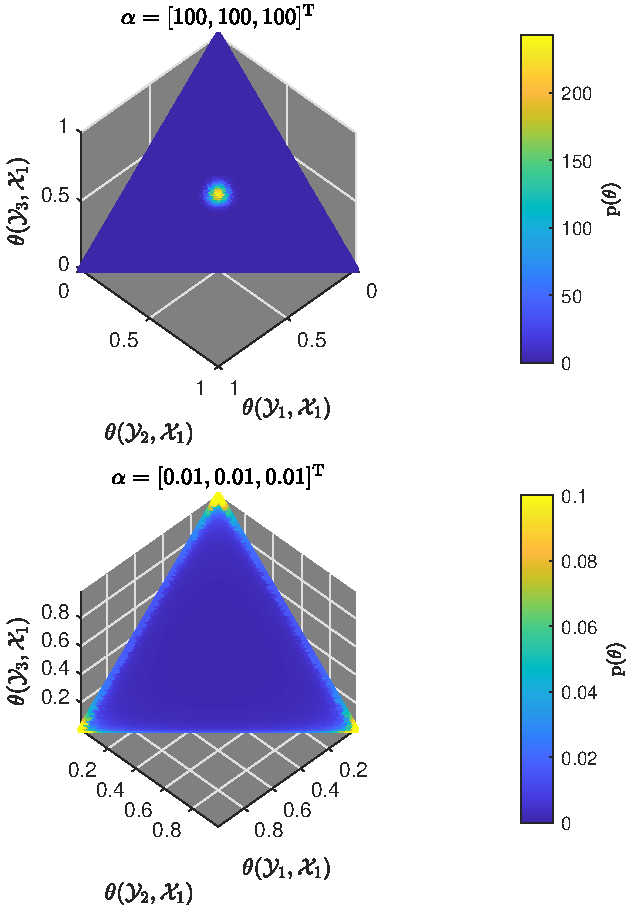
\includegraphics[scale=1.0]{P_theta.pdf}
\caption{Prior distributions for $\bar{\bm{\theta}}$ and $\bm{\theta}$, $M=3$}
\label{fig:P_theta}
\end{figure}


\subsubsection{Training data marginal PMF, $\text{P}(D)$}

Next we determine $\text{P}(D)$ -- extension to the joint distribution is straightfoward. Our starting point is expression of the PDF via the conditional independence of the training data for a given model $\bm{\theta}$,

\begin{equation}
\text{P}(D) = \int_{\bm{\Theta}} \left[ \prod_{n=1}^N \text{P}(D(n) | \bm{\theta}) \right] \text{p}(\bm{\theta}) \mathrm{d}\bm{\theta} \;.
\end{equation}

Since $\text{P}(D(n) = y_m | \bm{\theta}) = \theta_m$, we can simplify the PMF to,

\begin{equation} \label{P_D_int2}
\text{P}(D) = \int_{\bm{\Theta}} \left[ \prod_{m=1}^M \bm{\theta}_m^{\bar{N}_m(D)} \right] \text{p}(\bm{\theta}) \mathrm{d}\bm{\theta} 
= \text{E}_{\bm{\theta}} \left[ \prod_{m=1}^M \bm{\theta}_m^{\bar{N}_m(D)} \right] \;,
\end{equation}

where we have introduced a new vector random variable $\bar{\bm{\mathrm{n}}} = \bar{\bm{N}}(\mathrm{D})$ (sufficient statistic???) via transform function $\bar{\bm{N}}: \mathcal{Y}^N \mapsto \bar{\mathcal{N}} = \left\{ \bar{\bm{n}} \in \mathbb{N}^M: \sum_{m=1}^M \bar{\bm{n}}_m = N \right\}$, which is defined as,

%where we have introduced a new random variable (sufficient statistic???) $\bar{\bm{\mathrm{N}}} \in \bar{\bm{\mathcal{N}}} = \left\{ \bar{\bm{N}} \in \mathbb{N}^M: \sum_{m=1}^M \bar{\bm{N}}_m = N \right\}$ via transform function $\bar{\bm{N}}: \mathcal{Y}^N \mapsto \left\{ \bar{\bm{N}}??? \in \mathbb{N}^M: \sum_{m=1}^M \bar{\bm{N}}_m = N \right\}$, which is defined as,

\begin{equation}
\bar{N}_m(D) = \sum_{n=1}^N \delta[D(n),y_m] \;,
\end{equation}

where $\delta[\cdot,\cdot]$ is the Kronecker delta function. Observe that $\text{P}(D)$ can be interpreted as a joint moment of $\bm{\theta}$. Also, note the dimensionality reduction from $N$ to $M$ SET SIZE??? provided by the transformation. Finally, as detailed in Appendix \ref{app:P_D}, the training data PMF reduces to,

\begin{equation} \label{P_D}
\text{P}(D) = \binom{N+M-1}{\bar{N}_1(D),\ldots,\bar{N}_M(D),M-1}^{-1} 
= \binom{N+M-1}{N,M-1}^{-1} \binom{N}{\bar{N}_1(D),\ldots,\bar{N}_M(D)}^{-1} \;.
\end{equation}

Note the use of multinomial and binomial coefficients, as well as the functional dependence on $\mathrm{D}$ only through $\bar{\bm{N}}$. It should be clear that since the PDF is inversely proportionate to the multinomial coefficient of $\bar{\bm{N}}$, training data sets are more probable when they are more ``concentrated''. 





\subsubsection{Output conditional PMF, $\text{P}(y | D)$}

Equation \eqref{P_D} can be used to illuminate the forms of all the PMF's of interest, namely $\text{P}(y)$, $\text{P}(y,D)$, and $\text{P}(y | D)$.  $\text{P}(y)$ follows immediately by evaluating $\text{P}(D)$ for $N=1$, leading to a uniform PMF,

\begin{equation}
\text{P}(y_m) = \text{E}[\theta_m] = M^{-1}, \qquad m=1,\ldots,M \;.
\end{equation}

The joint distribution between $\mathrm{y}$ and $\mathrm{D}$ is expressed by simply extending $\text{P}(D)$ to $N+1$ data and treating $y$ separately in the multinomial coefficient:

\begin{equation} \label{P_yD}
\text{P}(y_m,D) = \binom{N+M}{\ldots,\bar{N}_{m-1}(D),\bar{N}_m(D)+1,\bar{N}_{m+1}(D),\ldots,M-1}^{-1} \;.
\end{equation}

Combining previous results, the PMF of the unobserved output conditioned on the training set is,

\begin{equation} \label{P_y_D_basic}
\text{P}(y_m | D) = \frac{\text{P}(y_m,D)}{\text{P}(D)} = \frac{\bar{N}_m(D)+1}{N+M} \;.
\end{equation}

A more interesting form for the conditonal PMF is,

%\begin{equation} \label{P_y_D}
%\text{P}(y_m | D) = \left(\frac{M}{N+M}\right) M^{-1} + \left(\frac{N}{N+M}\right) \frac{\bar{N}_m(D)}{N} \;.
%\end{equation}

\begin{IEEEeqnarray}{rCl} \label{P_y_D}
\text{P}(y_m | D) & = & \left(\frac{M}{N+M}\right) M^{-1} + \left(\frac{N}{N+M}\right) \frac{\bar{N}_m(D)}{N} \\
& = & \left(\frac{M}{N+M}\right) M^{-1} + \left(\frac{N}{N+M}\right) N^{-1}\sum_{n=1}^N \delta[D(n),y_m] \;.
\end{IEEEeqnarray}

FIGURE EX????

Observe how the terms in parentheses act as weighting factors providing a convex combination of two distributions: a uniform distribution independent of the data (specifically, $\text{P}(y_m) = \text{E}[\theta_m]$) and an empirical distribution independent of any prior knowledge.

The asymptotic behavior of this conditional PMF if of specific interest. As the cardinality $|\mathcal{Y}| = M$ increases relative to the number of training samples $N$, the PMF trends towards a uniform, ``uninformative'' distribution. Conversely, as the number of training points increases towards infinity, the PMF trends towards the empirical distribution. 






\subsubsection{Model Posterior, $\text{P}(\bm{\theta} | D)$}

Although we have already found the posterior PMF $\text{P}(y | D)$ via Bayes theorem, it is informative to consider another approach using a ``hidden'' distribution: the model posterior PMF, $\text{p}(\bm{\theta} | D)$. 

As mentioned previously, $\mathrm{y}$ and $\mathrm{D}$ have the property of conditional independence given the model; as such, $\text{P}(y,D) = \text{E}_{\bm{\theta}} \left[ \text{P}(y | \bm{\theta}) \text{P}(D | \bm{\theta}) \right]$. This enables the following interpretation of the PMF of $\mathrm{y}$ conditioned on the observed training data:

\begin{equation}
\text{P}(y_m | \mathrm{D}) = \text{E}_{\bm{\theta} | \mathrm{D}} \left[ \text{P}(y_m|\bm{\theta}) \right] = \text{E}\left[ \theta_m | \mathrm{D} \right] \;.
\end{equation}

As such, the posterior PMF $\text{P}(y | D)$ can we thought of as the expected value of $\bm{\theta}$ given the training data. This should be intuitively satisfying -- before observing the training set, the PMF of $y$ is simply $\text{E}[\bm{\theta}]$; the observations simply refine the distribution of the unknown model. Using previous results, we express the model posterior PMF in closed form as shown below. Graphical examples are provided in Figure \ref{fig:P_theta_D}.

\begin{equation} \label{P_t_D}
\text{p}(\bm{\theta} | D) = \frac{\text{P}(D | \bm{\theta}) \text{p}(\bm{\theta})}{\text{P}(D)}
= (N+M-1)! \prod_{m=1}^M \frac{\theta_m^{\bar{N}_m(D)}}{\bar{N}_m(D)!} ,  \quad  \forall \bm{\theta} \in \bm{\Theta} \;.
\end{equation}


In the machine learning literature, the model posterior is of specific interest. A popular use of the distribution is to form a point estimate of the model $\bm{\theta}$ by finding the maximizing value of the distribution - the resultant estimate is known as the Maximum \emph{a posteriori} (MAP) estimate. 

As shown in Appendix \ref{app:MAP_theta}, the MAP estimator is,

\begin{equation}
\hat{\bm{\theta}}_{MAP}(D) = \argmax_{\bm{\theta} \in \bm{\Theta}} \text{P}(\bm{\theta} | D) = \frac{\bar{\bm{N}}(D)}{N} \;,
\end{equation}

which is the same empirical distribution seen in equation \eqref{P_y_D}. Additionally, because $\text{P}(\bm{\theta})$ is uniform, the MAP estimator is equivalent to the Maximum Likelihood (ML) estimate $\hat{\bm{\theta}}_{ML}(D) = \argmax_{\bm{\theta} \in \bm{\Theta}} \text{P}(D | \bm{\theta})$, which is commonly used for non-Bayesian treatments of parameter estimation.


Next, we will provide the first and second moments of the conditional distribution and give some informative examples to show how the training data ``sharpens'' the non-informative distribution $\text{p}(\bm{\theta})$. Using equations \eqref{P_y_D_basic} and \eqref{P_y_D}, we can compactly display the mean of $\text{p}(\bm{\theta} | D)$ as,

\begin{equation}
\mu_{\bm{\theta} | D} \equiv \text{E}[\bm{\theta} | D] = \frac{\bar{\bm{N}}(D)+1}{N+M} = \left(\frac{M}{N+M}\right) M^{-1} + \left(\frac{N}{N+M}\right) \frac{\bar{\bm{N}}(D)}{N} \;.
\end{equation}

The second moments are generated in Appendix \ref{app:cov_theta_D}; combining with the mean above, we find the covariance matrix of $\bm{\theta}$ given $D$,

\begin{IEEEeqnarray}{rCl} 
\Sigma_{\bm{\theta} | D} & \equiv & \text{E}_{\bm{\theta} | D} \left[ (\bm{\theta} - \mu_{\bm{\theta} | D}) (\bm{\theta} - \mu_{\bm{\theta} | D})^\text{T} \right] \\ 
& = & \frac{\text{diag}(\bar{\bm{N}}(D) + \bm{1})}{(N+M+1)(N+M)} - \frac{(\bar{\bm{N}}(D) + \bm{1}) (\bar{\bm{N}}(D) + \bm{1})^\text{T}}{(N+M+1)(N+M)^2} \;. \label{cov_theta_D}
\end{IEEEeqnarray}

Comparing the numerators and denominators in the above expression, it is clear that as the size of the training set $N$ trends toward infinity, the variance of the model trends to zero. When also considering the limiting forms of $\mu_{\bm{\theta} | D}$, we observe that,

\begin{equation}
\text{p}(\bm{\theta} | D) \longrightarrow \delta \left( \bm{\theta} - \frac{\bar{\bm{N}}(D)}{N} \right) \;,
\end{equation}

or we converge in the mean-square sense???? In distribution??? Thus, with infinite training data, the generative model $\bm{\theta}$ can be determined precisely and used to determine the optimal learning function. 

\begin{figure}
\centering
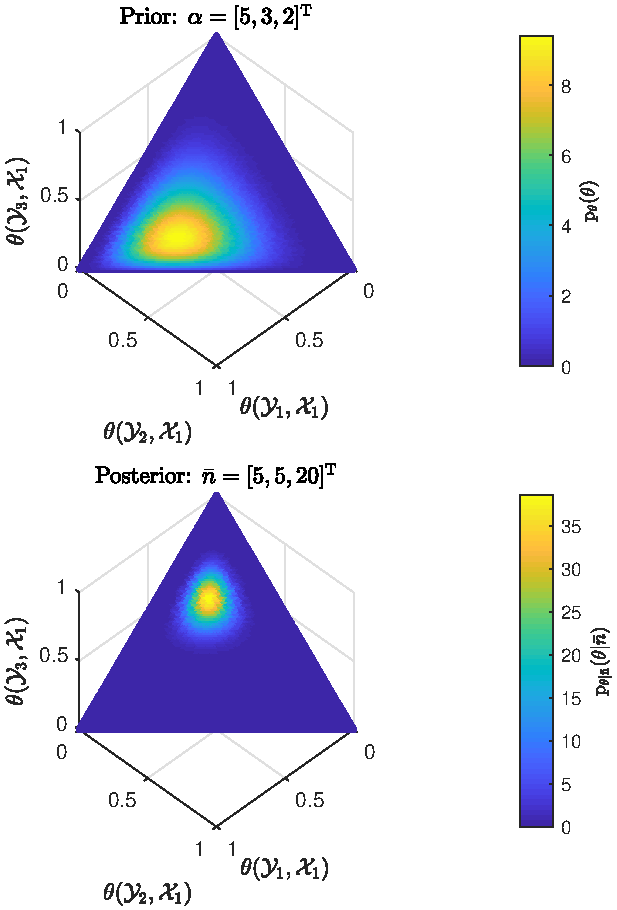
\includegraphics[scale=1.0]{P_theta_post.pdf}
\caption{Posterior model PDF's for various training sets $D$}
\label{fig:P_theta_D}
\end{figure}



\section{Application to Common Loss Functions}

In this section, we will proceed to apply the previous results to determine specific optimal learners and assess performance for two of the most common loss functions in machine learning: the squared error function, common for regression problems, and the 0-1 function, common for classification problems. Noting again the significance of $\text{P}(y|D)$ in finding the optimal learner in equation \eqref{f_opt_D}, and using \eqref{P_y_D}, we have,

\begin{IEEEeqnarray}{rCl}
\text{E}_{\mathrm{y} | \mathrm{D}} [ \mathcal{L}(h,\mathrm{y}) ] & = & \sum_{m=1}^M \mathcal{L}(h,y_m) \text{P}(y_m | \mathrm{D}) \\
& = & \left( \frac{M}{N+M} \right) M^{-1} \sum_{m=1}^M \mathcal{L}(h,y_m) +  \left( \frac{N}{N+M} \right) \sum_{m=1}^M \mathcal{L}(h,y_m) \frac{\bar{N}_m(D)}{N} \\
& = & \left( \frac{M}{N+M} \right) M^{-1} \sum_{m=1}^M \mathcal{L}(h,y_m) +  \left( \frac{N}{N+M} \right) N^{-1} \sum_{n=1}^N \mathcal{L}(h,D(n)) \;.
\end{IEEEeqnarray}

Note that by using the mixed distribution of \eqref{P_y_D}, we split the risk into a convex combination of two expected losses. Furthermore, by substituting in the formula for $\bar{\bm{N}}(D)$, we show the second expectation to be equivalent to the empirical loss.




\subsection{Classification: the 0-1 Loss}
In this section, we will apply the developed framework to the machine learning problem to which it is most applicable: classification. In classification problems, the hidden variable space is countable and almost always finite. Furthermore, the hypothesis space  is usually identical to the unobserved variable space, that is $\mathcal{H} = \mathcal{Y}$. The 0-1 loss function is the most well known for these problems; it is represented as,

\begin{equation} \label{loss_01}
\mathcal{L}(h,y) = 1 - \delta[h,y] \;.
\end{equation}

\subsubsection{Optimal Learner: the MAP class}

To determine the optimal learning function $f$, we combine the loss function \eqref{loss_01} with the posterior PMF of equation \eqref{P_y_D_basic}; the conditional expected loss reduces to,

\begin{IEEEeqnarray}{rCl}
\text{E}_{\mathrm{y} | \mathrm{D}} [ \mathcal{L}(h_m,\mathrm{y}) ] & = & 1 - \text{P}_{\mathrm{y} | \mathrm{D}}(h_m | \mathrm{D}) \\
& = & 1 - \left( \frac{M}{N+M} \right) M^{-1} - \left( \frac{N}{N+M} \right) \frac{\bar{N}_m(D)}{N} \;.  
\end{IEEEeqnarray}

Substituting into equation \eqref{f_opt_D}, the optimal learning function can be expressed as,

\begin{IEEEeqnarray}{rCl}
f^*(\mathrm{D}) & = & \argmin_{h \in \mathcal{Y}} \text{E}_{\mathrm{y} | \mathrm{D}}\left[ 1 - \text{P}_{\mathrm{y} | \mathrm{D}}(h_m | \mathrm{D})  \right] \\
& = & \argmax_{h \in \mathcal{Y}} \text{P}_{\mathrm{y} | \mathrm{D}}(h | \mathrm{D}) \;,
\end{IEEEeqnarray}

or, more simply,

\begin{equation}
f^*(\mathrm{D}) = y_{m^*},  \quad \text{where } m^* = \argmax \bar{N}_m(\mathrm{D}) \;.
\end{equation}

Given our lack of prior preference in any of the PMF's $\bm{\theta}$, the best class estimate is simply found by choosing the class most represented in the training set $D$.


\subsubsection{Minimum Risk: the Probability of Error}
Starting from equation \eqref{risk_min}, we formulate the minimum risk as,

\begin{IEEEeqnarray}{rCl}
\mathcal{R}(f^*) & = & \text{E}_{\mathrm{D}} \left[ \text{E}_{\mathrm{y} | \mathrm{D}} [ \mathcal{L}(f^*(\mathrm{D}),\mathrm{y}) ] \right]
= 1 - \text{E}_{\mathrm{D}} \left[ \max_{y} \text{P}_{\mathrm{y} | \mathrm{D}}(y | \mathrm{D}) \right] \\
& = & 1 - \text{E}_{\mathrm{D}} \left[ \frac{\max_m \bar{N}_m(D) + 1}{N+M} \right] \\\
& = & 1 - \left( \frac{M}{N+M} \right) M^{-1} - \left( \frac{N}{N+M} \right) \frac{\text{E}_\mathrm{D} \left[ \max_m \bar{N}_m(\mathrm{D}) \right]}{N} \;. \label{risk_01_opt}
\end{IEEEeqnarray}

To find a closed-form expression, we must evaluate the expectation over all possible training sets $D$. It can be clearly shown that the expectation can instead be performed over random variable $\bar{\bm{\mathrm{n}}} = \bar{\bm{N}}(\mathrm{D})$, that is,

\begin{equation}
\text{E}_\mathrm{D} \left[ \max_m \bar{N}_m(\mathrm{D}) \right] = \text{E}_{\bar{\bm{n}}} \left[ \max_m \bar{\mathrm{n}}_m \right] \;.
\end{equation}

In Appendix \ref{app:E_N_max}, we generate the cumulative mass function (CMF) of $\bar{\mathrm{n}}_{\text{max}} \equiv \max_m \bar{\mathrm{n}}_m$, 

\begin{IEEEeqnarray}{rCl}
F_{\bar{\mathrm{n}}_{\text{max}}}(n) & = & \text{P}\left( \bar{\mathrm{n}}_{\text{max}} \leq n \right) \\
& = & \binom{N+M-1}{M-1}^{-1} \sum_{m=1}^M \binom{M}{m} (-1)^{M-m} \\
&& \quad \binom{m(n+1)-N-1}{M-1} U\left(n+1-\frac{N+M}{m}\right) \;.
\end{IEEEeqnarray}

where $U: \mathbb{R} \mapsto \{0,1\}$ is the continuous step function. The expected value is thus,

\begin{IEEEeqnarray}{rCl}
\text{E}_{\bar{\bm{n}}} \left[ \bar{\mathrm{n}}_{\text{max}} \right] & = & \sum_{n=0}^N n \left( F_{\bar{\mathrm{n}}_{\text{max}}}(n) - F_{\bar{\mathrm{n}}_{\text{max}}}(n-1) \right) \\
& = & N - \sum_{n=0}^{N-1} F_{\bar{\mathrm{n}}_{\text{max}}}(n) \\
& = & N - \binom{N+M-1}{M-1}^{-1} \sum_{m=1}^M \binom{M}{m} (-1)^{M-m} \\
&& \quad \sum_{n = \left\lceil \frac{N+M}{m} \right\rceil}^N \binom{mn-N-1}{M-1} \;.
\end{IEEEeqnarray}

Although this form has not been reduced further, we can find a more compact form in the limit of training set volume, $N \to \infty$. As detailed in Appendix \ref{app:E_N_max},

\begin{equation}
\lim_{N \to \infty} \frac{\text{E}_{\bar{\bm{n}}} \left[ \max_m \bar{n}_m \right]}{N} = \frac{1}{M} \sum_{m=1}^M \frac{1}{m} \;.
\end{equation}

Note that this summation has no closed-form -- it is a Harmonic number REF???? Note also that if the class set is countably infinite, this summation can be represented as,

\begin{equation}
\lim_{M \to \infty} \frac{1}{M} \sum_{m=1}^M \frac{1}{m} = \frac{\text{ln}(M)}{M} \;.
\end{equation}

Substituting this formula into equation \eqref{risk_01_opt}, we determine the optimal risk,

\begin{equation}
\lim_{N \to \infty} \mathcal{R}(f^*)  = \lim_{N \to \infty} \left( 1 - \frac{\text{E}_\mathrm{D} \left[ \max_m \bar{N}_m(\mathrm{D}) \right]}{N} \right) = 1 - \frac{1}{M} \sum_{m=1}^M \frac{1}{m} \;,
\end{equation}

providing a lower bound to the risk that any learner can achieve with any volume of training data. Figure \ref{fig:Risk_01_opt} displays this risk, as well as the optimal risk when no training data is available.


FIGURES???
\begin{figure}
\centering
\includegraphics[scale=1.0]{Risk_01_opt.pdf}
\caption{Optimal 0-1 Risk}
\label{fig:Risk_01_opt}
\end{figure}


\subsection{Regession: the Squared-Error Loss}

The squared-error (SE) loss function is by far the most popular loss function for regression, or in fact any estimation problems where the variable of interest is continuous. This is due to its convexity, which allows easy determination of the minimizing function. We add an important generalization to this problem: we allow the estimate $\hat{y}$ DIFFERENT NOTATION???? to exist in a space that may differ from the space $\Omega$ of unobserved $y$. Such an approach is common in classification and general decision theory; here, we want to allow the variable to exist in a contiuous space to enable the closed-form solution for the minimizing solution.









\appendix


\section{Hypervolume of $\bar{\bm{\Theta}}$} \label{app:Theta}

INDUCTION PROOF??

To determine the value of the uniform PDF of $\bm{\theta}$, we must find the hypervolume of the set $\bar{\bm{\Theta}}$ for any cardinality $|\mathcal{Y}| = M$. First, we define the hypervolume of a modified set,

\begin{equation}
V_M(x) = \left| \left\{ \bar{\bm{\theta}} \in {\mathbb{R}^+}^{M}: \sum_{m=1}^{M} \bar{\theta}_m \leq x \right\} \right| \;.
\end{equation}

Clearly, $V_1(x) = x$. We continue by defining $V_2(x)$ as a function of $V_1(x)$, and so on, such that,

\begin{equation}
V_M(x) = \int_0^x V_{M-1}(y) \mathrm{d}y \;.
\end{equation}

Straightforward application of the power rule of integration demonstrates that $V_M(x) = \frac{x^M}{M!}$. By evaluating at $x=1$, we have the desired hypervolume; the model PDF immediately follows,

\begin{equation}
\text{p}\left(\bar{\bm{\theta}}\right)= (M-1)!,  \quad \forall \bar{\bm{\theta}} \in \bar{\bm{\Theta}} \;.
\end{equation}




\section{PMF of training data, $\mathrm{D}$} \label{app:P_D}

To develop the PMF form displayed in equation \eqref{P_D}, we first find the PMF of the transformed random variable, $\bar{\bm{\mathrm{n}}}$. Next, we leverage the dependency of $\text{P}(D)$ on the training data only through $\bar{\bm{\mathrm{n}}} = \bar{\bm{N}}(\mathrm{D})$ to arrive at the desired form.

We demonstrate that the PMF of $\bar{\bm{\mathrm{n}}}$ is uniform over the set $\bar{\mathcal{N}} = \left\{ \bar{\bm{n}} \in \mathbb{N}^M: \sum_{m=1}^M \bar{n}_m = N \right\}$. Our starting point leverages equation \eqref{P_D_int2} and the rule for transformation of random variables:

\begin{IEEEeqnarray}{rCl} \label{P_Nbar_int}
\text{P}_{\bar{\bm{\mathrm{n}}}}(\bar{\bm{n}}) & = & \sum_{ \{D\in\mathcal{D}: \bar{\bm{N}}(D) = \bar{\bm{n}}\} } \text{P}(D) = \left| \{D\in\mathcal{D}: \bar{\bm{N}}(D) = \bar{\bm{n}}\} \right| \cdot  g(\bar{\bm{n}}) \\
& = & \binom{N}{\bar{n}_1,\ldots,\bar{n}_M} \int_{\bm{\Theta}} \left[ \prod_{m=1}^M \theta_m^{\bar{n}_m} \right] \text{p}(\bm{\theta}) \mathrm{d}\bm{\theta} \;.
\end{IEEEeqnarray}

%\subsection{The PMF of $\bar{\bm{\mathrm{n}}} = \bar{\bm{N}}(\mathrm{D})$}

\subsection{Permutation invariance of $\text{P}_{\bar{\bm{\mathrm{n}}}}(\bar{\bm{n}})$}

Herer, we introduce a general permutation operator $\bm{H}: \bar{\mathcal{N}} \mapsto \bar{\mathcal{N}}$. Note that the operation is linear and invertible; using linear algebra, we consider matrix $\bm{H} \in \{0,1\}^{M \times M}$ and note that $\text{det}(\bm{H}) = 1$. Also, observe that $\bar{\mathcal{N}} = \{ \bm{H}\bar{\bm{n}} : \bar{\bm{n}} \in \bar{\mathcal{N}} \}$ -- the set is ``invariant'' to permutations. Now, we proceed to establish the uniformity of $\text{P}(\bar{\bm{n}})$ by proving two properties. 


First, we show that the PMF is also invariant to permutations of its argument $\bar{\bm{n}}$. In the following, we use the properties established above and a change of variables, $\bm{\phi} = \bm{H}^{-1} \bm{\theta}$. Note that the set of models $\bm{\Theta}$ is also invariant to permutations.

\begin{IEEEeqnarray}{rCl}
\text{P}_{\bar{\bm{\mathrm{n}}}}(\bm{H} \bar{\bm{n}}) & = & \binom{N}{[\bm{H}\bar{\bm{n}}]_1,\ldots,[\bm{H}\bar{\bm{n}}]_M} (M-1)!
\int_{\bm{\Theta}} \prod_{m=1}^M \theta_m^{[\bm{H}\bar{\bm{n}}]_m} \mathrm{d}\bm{\theta} \\
& = & \binom{N}{\bar{n}_1,\ldots,\bar{n}_M} (M-1)! \int_{\{ \bm{H}^{-1}\bm{\theta} : \bm{\theta} \in \bm{\Theta} \}} 
\prod_{m=1}^M [\bm{H}\bm{\phi}]_m^{[\bm{H}\bar{\bm{n}}]_m} \text{det}(\bm{H})^{-1} \mathrm{d}\bm{\phi} \\
& = & \binom{N}{\bar{n}_1,\ldots,\bar{n}_M} (M-1)! \int_{\bm{\Theta}} 
\prod_{m=1}^M \phi_m^{\bar{n}_m} \mathrm{d}\bm{\phi} \\
& = & \text{P}_{\bar{\bm{\mathrm{n}}}}(\bar{\bm{n}}) \;.
\end{IEEEeqnarray}

\subsection{Iteration??}
Second, we show that $\text{P}_{\bar{\bm{\mathrm{n}}}} (\ldots,\bar{n}_{M-1},\bar{n}_{M}) = \text{P}_{\bar{\bm{\mathrm{n}}}} (\ldots,\bar{n}_{M-1}+1,\bar{n}_{M}-1)$. Expanding the integration, we have,

\begin{IEEEeqnarray}{rCl}
\text{P}_{\bar{\bm{\mathrm{n}}}}(\bar{\bm{n}}) & = & \binom{N}{\bar{n}_1,\ldots,\bar{n}_M} (M-1)! 
\int_0^{1} \theta_1^{\bar{n}_1} \int_0^{1-\theta_1} \theta_2^{\bar{n}_2} \ldots \\
&& \int_0^{1 - \sum_{m=1}^{M-2} \theta_m} \theta_{M-1}^{\bar{n}_{M-1}} \left( 1 - \sum_{m=1}^{M-1} \theta_m \right)^{\bar{n}_M} \mathrm{d}\bm{\theta} \;.
\end{IEEEeqnarray}

Performing integration by parts over $\theta_{M-1}$, we observe that,

\begin{IEEEeqnarray}{rCl}
\text{P}_{\bar{\bm{\mathrm{n}}}}(\bar{\bm{n}}) & = & \binom{N}{\bar{n}_1,\ldots,\bar{n}_M} (M-1)! 
\int_0^{1} \theta_1^{\bar{n}_1} \int_0^{1-\theta_1} \theta_2^{\bar{n}_2} \ldots \\
&& \frac{\bar{n}_M}{\bar{n}_{M-1}+1} \int_0^{1 - \sum_{m=1}^{M-2} \theta_m} \theta_{M-1}^{\bar{n}_{M-1}+1} \left( 1 - \sum_{m=1}^{M-1} \theta_m \right)^{\bar{n}_M-1} \mathrm{d}\theta_{M-1} \\
& = & \binom{N}{\ldots,\bar{n}_{M-1}+1,\bar{n}_M-1} (M-1)! \int_0^{1} \theta_1^{\bar{n}_1} \int_0^{1-\theta_1} \theta_2^{\bar{n}_2} \ldots \\
&& \int_0^{1 - \sum_{m=1}^{M-2} \theta_m} \theta_{M-1}^{\bar{n}_{M-1}+1} \left( 1 - \sum_{m=1}^{M-1} \theta_m \right)^{\bar{n}_M-1} \mathrm{d}\theta_{M-1} \\
& = & \text{P}_{\bar{\bm{\mathrm{n}}}} (\ldots,\bar{n}_{M-1}+1,\bar{n}_{M}-1) \;.
\end{IEEEeqnarray}

%\begin{IEEEeqnarray}{L}
%\int_0^{1 - \sum_{m=1}^{M-2} \theta_m} \theta_{M-1}^{\bar{n}_{M-1}} \left( 1 - \sum_{m=1}^{M-1} \theta_m \right)^{\bar{n}_M} \mathrm{d}\theta_{M-1} \\
%= \frac{\bar{n}_M}{\bar{n}_{M-1}+1} \int_0^{1 - \sum_{m=1}^{M-2} \theta_m} \theta_{M-1}^{\bar{n}_{M-1}+1} \left( 1 - \sum_{m=1}^{M-1} \theta_m \right)^{\bar{n}_M-1}\mathrm{d}\theta_{M-1} \;.
%\end{IEEEeqnarray}

Iterative application of this property shows that,

\begin{IEEEeqnarray}{rCl}
\text{P}_{\bar{\bm{\mathrm{n}}}} (\ldots,0,\bar{n}_{M-1} + \bar{n}_{M}) & = & \text{P}_{\bar{\bm{\mathrm{n}}}} (\ldots,1,\bar{n}_{M-1} + \bar{n}_{M}-1) \\
& = & \ldots = \text{P}_{\bar{\bm{\mathrm{n}}}} (\ldots,\bar{n}_{M-1} + \bar{n}_{M},0) \;.
\end{IEEEeqnarray}


\subsection{Uniformity of $\text{P}_{\bar{\bm{\mathrm{n}}}}(\bar{\bm{n}})$ and relation to $\text{P}(\mathrm{D})$}
Combining these properties, it is clear that all values of $\bar{\bm{n}}$ are equiprobable. Thus, the only remaining task is to determine the cardinality of $\bar{\mathcal{N}}$. Using the stars-and-bars method (REF WILLIAM FULLER???), we see that $|\bar{\mathcal{N}}| = \binom{N+M-1}{N,M-1}$. Finally, we have the PMF,

\begin{equation}
\text{P}_{\bar{\bm{\mathrm{n}}}} (\bar{\bm{n}}) = \binom{N+M-1}{N,M-1}^{-1}, \qquad \forall \bar{\bm{n}} \in \bar{\mathcal{N}} \;.
\end{equation}

Using \eqref{P_Nbar_int} and noting that $\left| \{D\in\mathcal{D}: \bar{\bm{N}}(D) = \bar{\bm{n}}\} \right| = \binom{N}{\bar{n}_1,\ldots,\bar{n}_M}$, we can solve for $g(\bar{\bm{n}})$, and immediately find,

\begin{IEEEeqnarray}{rCl}
\text{P}(D) & = & \binom{N+M-1}{N,M-1}^{-1} \binom{N}{\bar{N}_1(D),\ldots,\bar{N}_M(D)}^{-1} \\
& = & \binom{N+M-1}{\bar{N}_1(D),\ldots,\bar{N}_M(D),M-1}^{-1}
\end{IEEEeqnarray}




\section{Maximum \emph{a Posteriori} estimate of $\bm{\theta}$ given $D$} \label{app:MAP_theta}

To determine the MAP estimate of the model PMF $\bm{\theta}$ given the training data $D$, 

\begin{equation}
\hat{\bm{\theta}}_{MAP}(D) = \argmax_{\bm{\theta} \in \bm{\Theta}} \text{P}(\bm{\theta} | D) \;,
\end{equation}

we perform contrained optimization. Note that the set $\bm{\Theta} = \left\{ \bm{\theta} \in {\mathbb{R}^+}^{M}: \sum_{m=1}^{M} \theta_m = 1 \right\}$ implies both equality and inequality constraints -- to solve for the maximizing value of the model, we assess the Karush-Kuhn-Tucker (KKT) conditions REF BOYD??? using constraints $g_m(\bm{\theta}) = -\theta_m \leq 0, \quad \forall m = 1,\ldots,M$ and $h(\bm{\theta}) = \sum_{m=1}^M \theta_m = 1$. First, we mention that the regularity conditons are met, as all functions $g$ and $h$ are affine. Next we assess the necessary conditions; they are:

\begin{IEEEeqnarray}{C}
\nabla_{\bm{\theta}} \text{P}(\bm{\theta}^* | D) = \sum_{m=1}^M \mu_m \nabla_{\bm{\theta}} g_m(\bm{\theta}^*) + \lambda \nabla_{\bm{\theta}} h(\bm{\theta}^*) \label{MAP_t_st} \\ 
g_m(\bm{\theta}^*) = -\theta^*_m \leq 0, \quad \forall m = 1,\ldots,M \label{MAP_t_p_i} \\
h(\bm{\theta}^*) = \sum_{m=1}^M \theta^*_m = 1  \label{MAP_t_p_e} \\
\mu_m \geq 0, \quad \forall m = 1,\ldots,M \label{MAP_t_d} \\
\mu_m g_m(\bm{\theta}^*) = 0, \quad \forall m = 1,\ldots,M \label{MAP_t_cs}
\end{IEEEeqnarray}

PROOF STYLE??

Note the simplified notation -- dependence of the minimizer and of the KKT multipliers on training data $D$ is suppressed. We assert that $\bm{\theta}^*(D) = \frac{\bar{\bm{N}}(D)}{N}$, the empirical PMF. It is immediately clear that the emprical PMF satisfies the primal feasibility conditions \eqref{MAP_t_p_i} and \eqref{MAP_t_p_e}. Next, we show that the remaining conditions are met using KKT multipliers,

\begin{equation}
\mu_m(D) = \begin{cases} N \text{P}_{\bm{\theta} | D} \left( \frac{\bar{\bm{N}}(D)}{N} \right) & \text{if } \bar{N}_m(D) = 0, \\ 0 & \text{if } \bar{N}_m(D) > 0. \end{cases}
\end{equation}

\begin{equation}
\lambda(D) =  N \text{P}_{\bm{\theta} | D} \left( \frac{\bar{\bm{N}}(D)}{N} \right) \;.
\end{equation}

The formula for $\mu(D)$ satisfies the dual feasibility conditon \eqref{MAP_t_d} as well as the complementary slackness condition \eqref{MAP_t_cs}. To satisfy the stationarity condition \eqref{MAP_t_st}, note that,

\begin{equation}
\frac{\partial}{\partial \theta_m} \text{P}(\bm{\theta} | D) = \begin{cases} \bar{N}_m \theta_m^{-1} \text{P}(\bm{\theta} | D) & \text{if } \bar{N}_m(D) > 0, \\ 0 & \text{if } \bar{N}_m(D) = 0. \end{cases}
\end{equation}

It is straightforward to show that this final necessary conditon is met. Sufficient conditions??? Second order???

%To complete the proof, we mention that this optimization problem meets the requirements such that the necessary conditions are also sufficient. First, the constraint functions $g$ are convex (since they are affine), and $h$ is also affine. Second, $\text{P}(\bm{\theta} | D)$ 



%To simplify the proof, we will simply find the maximum over a different set $\bm{\Theta}' = \left\{ \bm{\theta} \in \mathbb{R}^M: \sum_{m=1}^{M} \theta_m = 1 \right\} \supset \bm{\Theta}$ and show that the maximimizing value over $\bm{\Theta}'$ is a member of $\bm{\Theta}$.
%
%Now with only equality constraints, we substitute in equation \eqref{P_t_D} for the posterior PDF and apply the method of Lagrange multipliers to find stationary points,
%
%\begin{IEEEeqnarray}{rCl}
%0 & = & \left. \frac{\partial}{\partial \theta_m} \left[ \text{P}(\bm{\theta} | D) + \lambda \left( \sum_{m=1}^M \theta_m - 1 \right) \right] \right|_{\bm{\theta} = \bm{\theta}^*} \\
%& = &  \bar{N}_m(D) {\theta_m^*}^{-1} \text{P}_{\bm{\theta} | D}(\bm{\theta}^* | D) + \lambda , \qquad m = 1,\ldots,M \;.
%\end{IEEEeqnarray}
%
%Rearranging and summing over $m$, we find $\lambda = -N \text{P}(\bm{\theta} | D)$. Finally,
%
%\begin{equation}
%\bm{\theta}^* = \frac{\bar{\bm{N}}}{N} \;.
%\end{equation}
%
%The single stationary point $\bm{\theta}^* \in {\mathbb{R}^+}^M$ and is thus a member of $\bm{\Theta}$ as well. To complete the proof, we must examine the second-order derivatives to confirm that the stationary point is the global maximum. To this effect, we use a bordered Hessian matrix,
%
%\begin{equation}
%\bm{H}(\bm{\theta},\lambda) = ??? = \begin{bmatrix} 0 & \bm{1}_{1 \times M} \\ \bm{1}_{M \times 1} & \text{P}(\bm{\theta}|D) \text{diag}(\bm{\theta})^{-1} \left( \bar{\bm{N}} \bar{\bm{N}}^{\text{T}} - \text{diag}(\bar{\bm{N}}) \right) \text{diag}(\bm{\theta})^{-1} \end{bmatrix} \;.
%\end{equation}
%
%\begin{equation}
%\left. \bm{H}(\bm{\theta},\lambda) \right|_{\bm{\theta}^*} = \begin{bmatrix} 0 & \bm{1}_{1 \times M} \\ \bm{1}_{M \times 1} & N^2 \text{P}(\bm{\theta}|D) \left( \bm{1}_{M \times M} - \text{diag}(\bar{\bm{N}})^{-1} \right) \end{bmatrix} \;.
%\end{equation}



\section{Covariance of $\text{P}(\bm{\theta}|D)$} \label{app:cov_theta_D}

To find the covariance of $\text{P}(\bm{\theta}|D)$, we must generate the second-order joint moments of the distribution. The approach used mirrors the one employed when we found the first moments, which we know are equivalent to $\text{P}(y|D)$. Observe that,

\begin{equation}
\text{E}[\theta_{m_1} \theta_{m_2} | D] = \frac{\int_{\bm{\Theta}} \theta_{m_1} \theta_{m_2} \left[ \prod_{m=1}^M \theta_m^{\bar{N}_m(D)} \right] \text{p}(\bm{\theta}) \mathrm{d}\bm{\theta}}{\text{P}(D)} \;.
\end{equation}

We have a closed-form expression for the denominator. To assess the numerator, we extend equation \eqref{P_yD} for an additional datum, such that,

\begin{equation}
\text{P}(y_{m_1},y_{m_2},D) = 
\begin{cases}
\binom{N+M+1}{\ldots,\bar{N}_{m_1-1}(D),\bar{N}_{m_1}(D)+2,\bar{N}_{m_1+1}(D),\ldots,M-1}^{-1} & \text{if } m_1 = m_2, \\ 
\binom{N+M+1}{\ldots,\bar{N}_{m_1-1}(D),\bar{N}_{m_1}(D)+1,\ldots,\bar{N}_{m_2}(D)+1,\bar{N}_{m_2+1}(D),\ldots,M-1}^{-1} & \text{if } m_1 \neq m_2.
\end{cases}
\end{equation}

Substituting in, the formula for the second moments becomes,

\begin{equation}
\text{E}[\theta_{m_1} \theta_{m_2} | D] =
\begin{cases}
\frac{(\bar{N}_{m_1}(D)+2)(\bar{N}_{m_1}(D)+1)}{(N+M+1)(N+M)} & \text{if } m_1 = m_2, \\  
\frac{(\bar{N}_{m_1}(D)+1)(\bar{N}_{m_2}(D)+1)}{(N+M+1)(N+M)} & \text{if } m_1 \neq m_2.
\end{cases}
\end{equation}

In vector form, this reduces to,

\begin{equation}
\text{E}[\bm{\theta} \bm{\theta}^\text{T} | D] = \frac{\text{diag}(\bar{\bm{N}}(D) + \bm{1})}{(N+M+1)(N+M)} + \frac{(\bar{\bm{N}}(D) + \bm{1}) (\bar{\bm{N}}(D) + \bm{1})^\text{T}}{(N+M+1)(N+M)} \;.
\end{equation}

Finally, we solve for equation \eqref{cov_theta_D} using $\Sigma_{\bm{\theta} | D} = \text{E}[\bm{\theta} \bm{\theta}^\text{T} | D] -  \mu_{\bm{\theta} | D}) \mu_{\bm{\theta} | D})^\text{T}$.




\section{The Expected Value of $\bar{\mathrm{n}}_{\text{max}}$} \label{app:E_N_max}

\subsection{The PMF of $\bar{\mathrm{n}}_{\text{max}}$}

???
FIGURES


\subsection{In the limit $N \to \infty$}

Having established the PMF for $\bar{\mathrm{n}}_{\text{max}}$ and provided a general formula for the expected value in equation ???, we seek a more tractable form to avoid the summation over $n=0,\ldots,N$. Although we do not provide the general expression, we do provide a compact formula for the expected value as $N \to \infty$.

First, we note how the CMF of $\bar{\mathrm{n}}_{\text{max}}$ simplifies in this limit. Below, observe how the binomial coefficients including $N$ reduce to a power term and that terms drop from the argument of the step function, which is invariant to scaling.

\begin{IEEEeqnarray}{rCl}
\lim_{N \to \infty} F_{\bar{\mathrm{n}}_{\text{max}}}(n) & = & \lim_{N \to \infty} \binom{N+M-1}{M-1}^{-1} \sum_{m=1}^M \binom{M}{m} (-1)^{M-m} \\
&& \quad \binom{m(n+1)-N-1}{M-1} U\left(n+1-\frac{N+M}{m}\right) \\
& = & \lim_{N \to \infty} \sum_{m=1}^M \binom{M}{m} (-1)^{M-m} U\left(\frac{n}{N}+\frac{1}{N}-\frac{1}{m}-\frac{M}{Nm}\right) \\
&& \quad \prod_{k=1}^M \frac{m(n+1)-N-k}{N+M-k} \\
& = & \lim_{N \to \infty} \sum_{m=1}^M \binom{M}{m} (-1)^{M-m} U\left( \frac{n}{N}-\frac{1}{m} \right) \left( \frac{mn}{N} - 1 \right)^{M-1} \\
\end{IEEEeqnarray}

Consider the dependency on $n$, as well as the presence of training set size $N$ in the above equation. We define a continuous function over the unit interval,

\begin{equation}
p(t) = \sum_{m=1}^M \binom{M}{m} (-1)^{M-m} (mt - 1)^{M-1} U\left( t-\frac{1}{m} \right) \;,
\end{equation}

such that $p(n/N) = \lim_{N \to \infty} F_{\bar{\mathrm{n}}_{\text{max}}}(n)$. This will be used in the following, where we use the CMF to determine the first moment. 

THETA PDF???

It should be intuitive that as $N$ trends toward infinity, so does $\text{E}_{\bar{\bm{n}}} \left[ \bar{\mathrm{n}}_{\text{max}} \right]$. With this expectation, and given the form of equation \eqref{risk_01_opt}, we proceed to determine the ``normalized'' value of the mean,

\begin{IEEEeqnarray}{rCl}
\lim_{N \to \infty} \frac{\text{E}_{\bar{\bm{n}}} \left[ \bar{\mathrm{n}}_{\text{max}} \right]}{N} & = & \lim_{N \to \infty} N^{-1} \sum_{n=0}^N n 
\left( F_{\bar{\mathrm{n}}_{\text{max}}}(n) - F_{\bar{\mathrm{n}}_{\text{max}}}(n-1) \right) \\
& = & \lim_{N^{-1} \to 0} N^{-1} \sum_{n=1}^N \frac{n}{N} \left( \frac{p(n/N) - p(n/N - N^{-1})}{N^{-1}} \right) \\
& = & \lim_{N^{-1} \to 0} N^{-1} \sum_{n=1}^N \frac{n}{N} \left. \frac{\mathrm{d}p(t)}{\mathrm{d}t} \right|_{t=n/N}  \\
& \approx & \int_0^1  t \frac{\mathrm{d}p(t)}{\mathrm{d}t} \mathrm{d}t \;,
\end{IEEEeqnarray}

where we represent the summation as a Riemann approximation of a tractable integration. Performing integration by parts, we have,

\begin{IEEEeqnarray}{rCl}
\lim_{N \to \infty} \frac{\text{E}_{\bar{\bm{n}}} \left[ \bar{\mathrm{n}}_{\text{max}} \right]}{N} & = & p(1) - \int_0^1 p(t) \mathrm{d}t \\
& = & 1 - \sum_{m=1}^M \binom{M}{m} (-1)^{M-m}
\end{IEEEeqnarray}


REF Knuth????


\section{Moments of N bar}

\end{document}


























